\documentclass[14pt]{extbook}
\usepackage{multicol, enumerate, enumitem, hyperref, color, soul, setspace, parskip, fancyhdr} %General Packages
\usepackage{amssymb, amsthm, amsmath, latexsym, units, mathtools} %Math Packages
\everymath{\displaystyle} %All math in Display Style
% Packages with additional options
\usepackage[headsep=0.5cm,headheight=12pt, left=1 in,right= 1 in,top= 1 in,bottom= 1 in]{geometry}
\usepackage[usenames,dvipsnames]{xcolor}
\usepackage{dashrule}  % Package to use the command below to create lines between items
\newcommand{\litem}[1]{\item#1\hspace*{-1cm}\rule{\textwidth}{0.4pt}}
\pagestyle{fancy}
\lhead{Progress Quiz 9}
\chead{}
\rhead{Version B}
\lfoot{9541-5764}
\cfoot{}
\rfoot{Summer C 2021}
\begin{document}

\begin{enumerate}
\litem{
Choose the equation of the function graphed below.
\begin{center}
    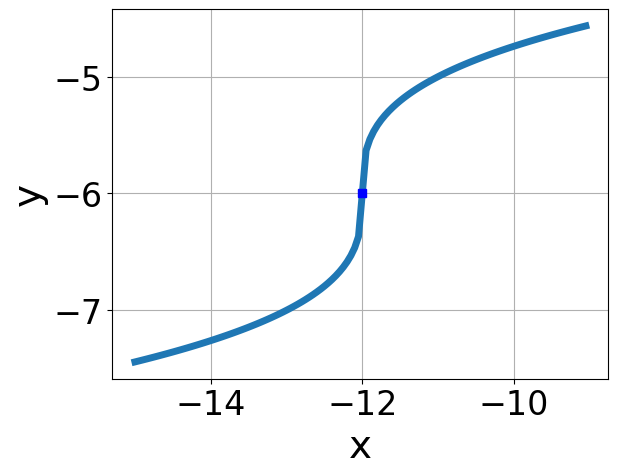
\includegraphics[width=0.5\textwidth]{../Figures/radicalGraphToEquationB.png}
\end{center}
\begin{enumerate}[label=\Alph*.]
\item \( f(x) = \sqrt{x + 12} - 6 \)
\item \( f(x) = \sqrt{x - 12} - 6 \)
\item \( f(x) = - \sqrt{x - 12} - 6 \)
\item \( f(x) = - \sqrt{x + 12} - 6 \)
\item \( \text{None of the above} \)

\end{enumerate} }
\litem{
Choose the equation of the function graphed below.
\begin{center}
    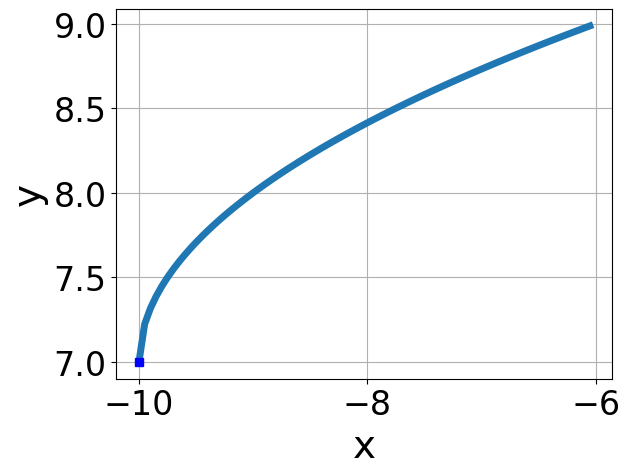
\includegraphics[width=0.5\textwidth]{../Figures/radicalGraphToEquationCopyB.png}
\end{center}
\begin{enumerate}[label=\Alph*.]
\item \( f(x) = - \sqrt{x - 10} + 7 \)
\item \( f(x) = \sqrt{x - 10} + 7 \)
\item \( f(x) = \sqrt{x + 10} + 7 \)
\item \( f(x) = - \sqrt{x + 10} + 7 \)
\item \( \text{None of the above} \)

\end{enumerate} }
\litem{
Solve the radical equation below. Then, choose the interval(s) that the solution(s) belongs to.\[ \sqrt{14 x^2 - 12} - \sqrt{-13 x} = 0 \]\begin{enumerate}[label=\Alph*.]
\item \( x \in [-2.71,-0.05] \)
\item \( x \in [-0.03,1.04] \)
\item \( x_1 \in [-0.03, 1.04] \text{ and } x_2 \in [1.18,2.2] \)
\item \( \text{All solutions lead to invalid or complex values in the equation.} \)
\item \( x_1 \in [-2.71, -0.05] \text{ and } x_2 \in [-0.34,0.79] \)

\end{enumerate} }
\litem{
Solve the radical equation below. Then, choose the interval(s) that the solution(s) belongs to.\[ \sqrt{5 x - 8} - \sqrt{8 x - 5} = 0 \]\begin{enumerate}[label=\Alph*.]
\item \( x \in [-3,0] \)
\item \( \text{All solutions lead to invalid or complex values in the equation.} \)
\item \( x_1 \in [-0.38, 5.62] \text{ and } x_2 \in [0.6,3.6] \)
\item \( x \in [-7.33,-1.33] \)
\item \( x_1 \in [-3, 0] \text{ and } x_2 \in [0.6,3.6] \)

\end{enumerate} }
\litem{
What is the domain of the function below?\[ f(x) = \sqrt[4]{-5 x + 8} \]\begin{enumerate}[label=\Alph*.]
\item \( (-\infty, \infty) \)
\item \( [a, \infty), \text{where } a \in [1.46, 1.79] \)
\item \( [a, \infty), \text{where } a \in [0.35, 1.05] \)
\item \( (-\infty, a], \text{where } a \in [0.2, 0.8] \)
\item \( (-\infty, a], \text{ where } a \in [1.2, 3] \)

\end{enumerate} }
\litem{
Choose the graph of the equation below.\[ f(x) = - \sqrt[3]{x - 8} + 4 \]\begin{enumerate}[label=\Alph*.]
\begin{multicols}{2}\item 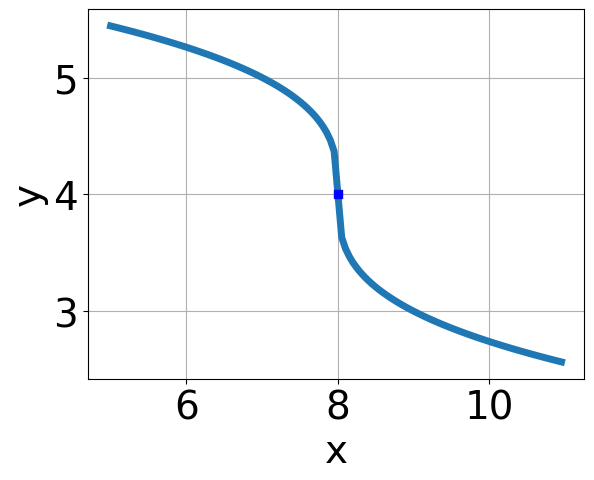
\includegraphics[width = 0.3\textwidth]{../Figures/radicalEquationToGraphAB.png}\item 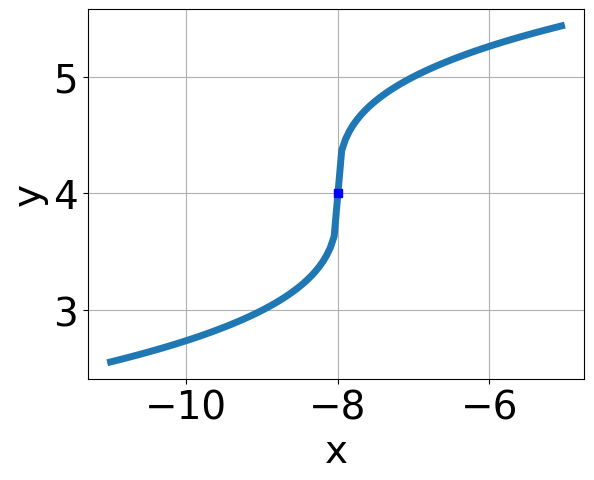
\includegraphics[width = 0.3\textwidth]{../Figures/radicalEquationToGraphBB.png}\item 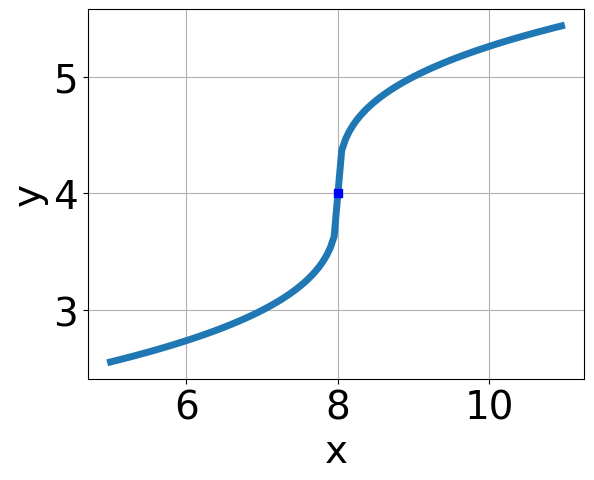
\includegraphics[width = 0.3\textwidth]{../Figures/radicalEquationToGraphCB.png}\item 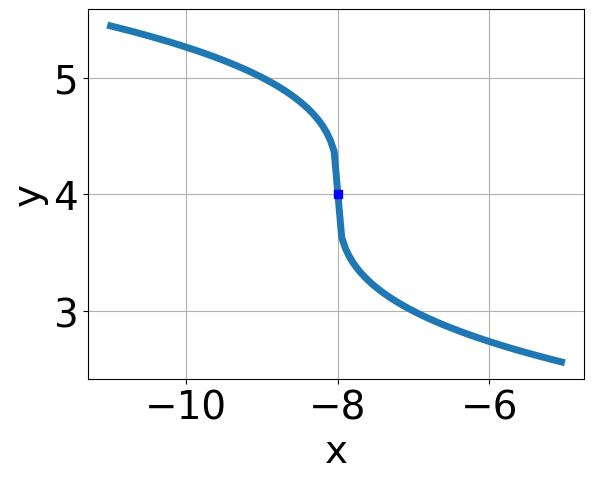
\includegraphics[width = 0.3\textwidth]{../Figures/radicalEquationToGraphDB.png}\end{multicols}\item None of the above.
\end{enumerate} }
\litem{
What is the domain of the function below?\[ f(x) = \sqrt[7]{8 x - 9} \]\begin{enumerate}[label=\Alph*.]
\item \( (-\infty, \infty) \)
\item \( \text{The domain is } [a, \infty), \text{   where } a \in [0.92, 1.31] \)
\item \( \text{The domain is } (-\infty, a], \text{   where } a \in [0.71, 1.01] \)
\item \( \text{The domain is } (-\infty, a], \text{   where } a \in [1.03, 1.25] \)
\item \( \text{The domain is } [a, \infty), \text{   where } a \in [0.86, 0.94] \)

\end{enumerate} }
\litem{
Solve the radical equation below. Then, choose the interval(s) that the solution(s) belongs to.\[ \sqrt{9 x^2 + 6} - \sqrt{15 x} = 0 \]\begin{enumerate}[label=\Alph*.]
\item \( x \in [0.2,0.91] \)
\item \( x_1 \in [0.2, 0.91] \text{ and } x_2 \in [0.3,4.3] \)
\item \( x \in [0.98,1.04] \)
\item \( x_1 \in [-1.07, -0.43] \text{ and } x_2 \in [-2.5,0.1] \)
\item \( \text{All solutions lead to invalid or complex values in the equation.} \)

\end{enumerate} }
\litem{
Choose the graph of the equation below.\[ f(x) = \sqrt{x - 10} + 4 \]\begin{enumerate}[label=\Alph*.]
\begin{multicols}{2}\item 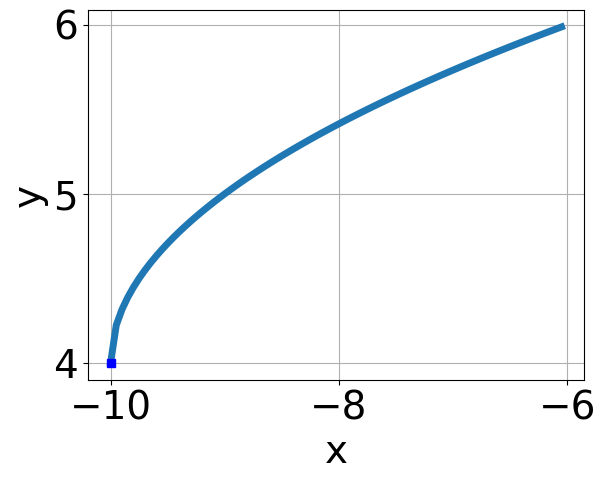
\includegraphics[width = 0.3\textwidth]{../Figures/radicalEquationToGraphCopyAB.png}\item 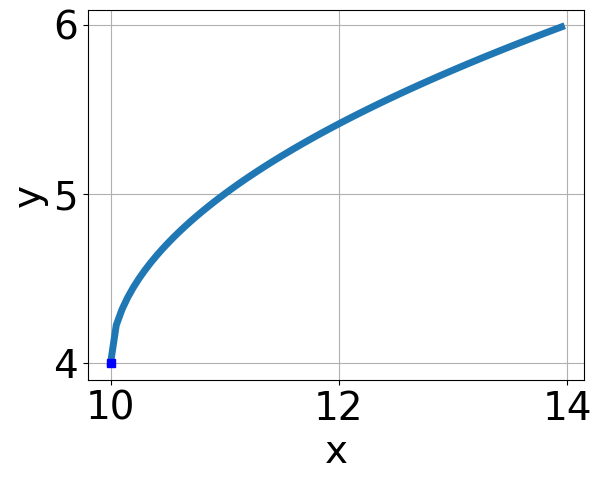
\includegraphics[width = 0.3\textwidth]{../Figures/radicalEquationToGraphCopyBB.png}\item 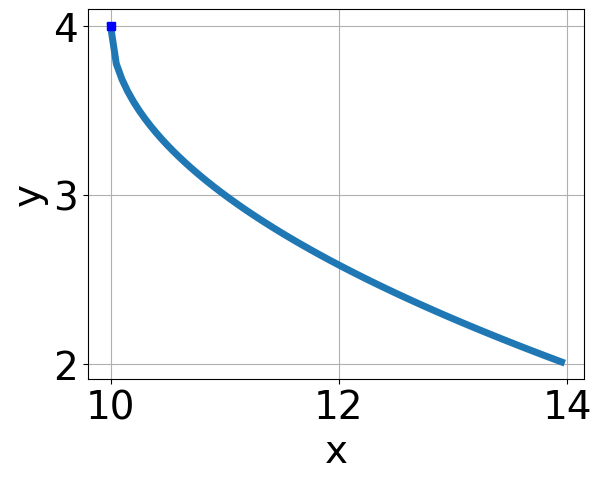
\includegraphics[width = 0.3\textwidth]{../Figures/radicalEquationToGraphCopyCB.png}\item 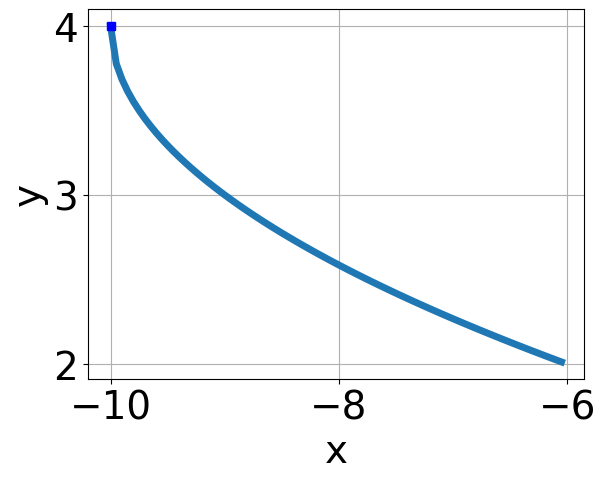
\includegraphics[width = 0.3\textwidth]{../Figures/radicalEquationToGraphCopyDB.png}\end{multicols}\item None of the above.
\end{enumerate} }
\litem{
Solve the radical equation below. Then, choose the interval(s) that the solution(s) belongs to.\[ \sqrt{8 x + 8} - \sqrt{-2 x + 7} = 0 \]\begin{enumerate}[label=\Alph*.]
\item \( x \in [-2.14,-1.24] \)
\item \( x \in [-0.76,0] \)
\item \( x_1 \in [-1.48, -0.65] \text{ and } x_2 \in [1.5,6.5] \)
\item \( \text{All solutions lead to invalid or complex values in the equation.} \)
\item \( x_1 \in [-1.48, -0.65] \text{ and } x_2 \in [-0.1,1.9] \)

\end{enumerate} }
\end{enumerate}

\end{document}